\section{Kapitel 1: Modellierung eines Leistungselektronik-Wandlers in PLECS} \label{sec:Task1}

Die Modellierung des Leistungselektronik-Wandlers ist ein zentraler Schritt zur Systemanalyse und Regelung. In diesem Kapitel wird die theoretische Grundlage erläutert, das Modell detailliert beschrieben und die Wahl der Modellstruktur sowie deren Auswirkungen auf das dynamische Verhalten diskutiert. Mögliche Vereinfachungen zur effizienten Implementierung des Reglers werden ebenfalls betrachtet. (Siehe Abbildung: \ref{fig:ControllerSoft} und \ref{fig:SystemSoft})

\begin{figure}[H]
    \centering
    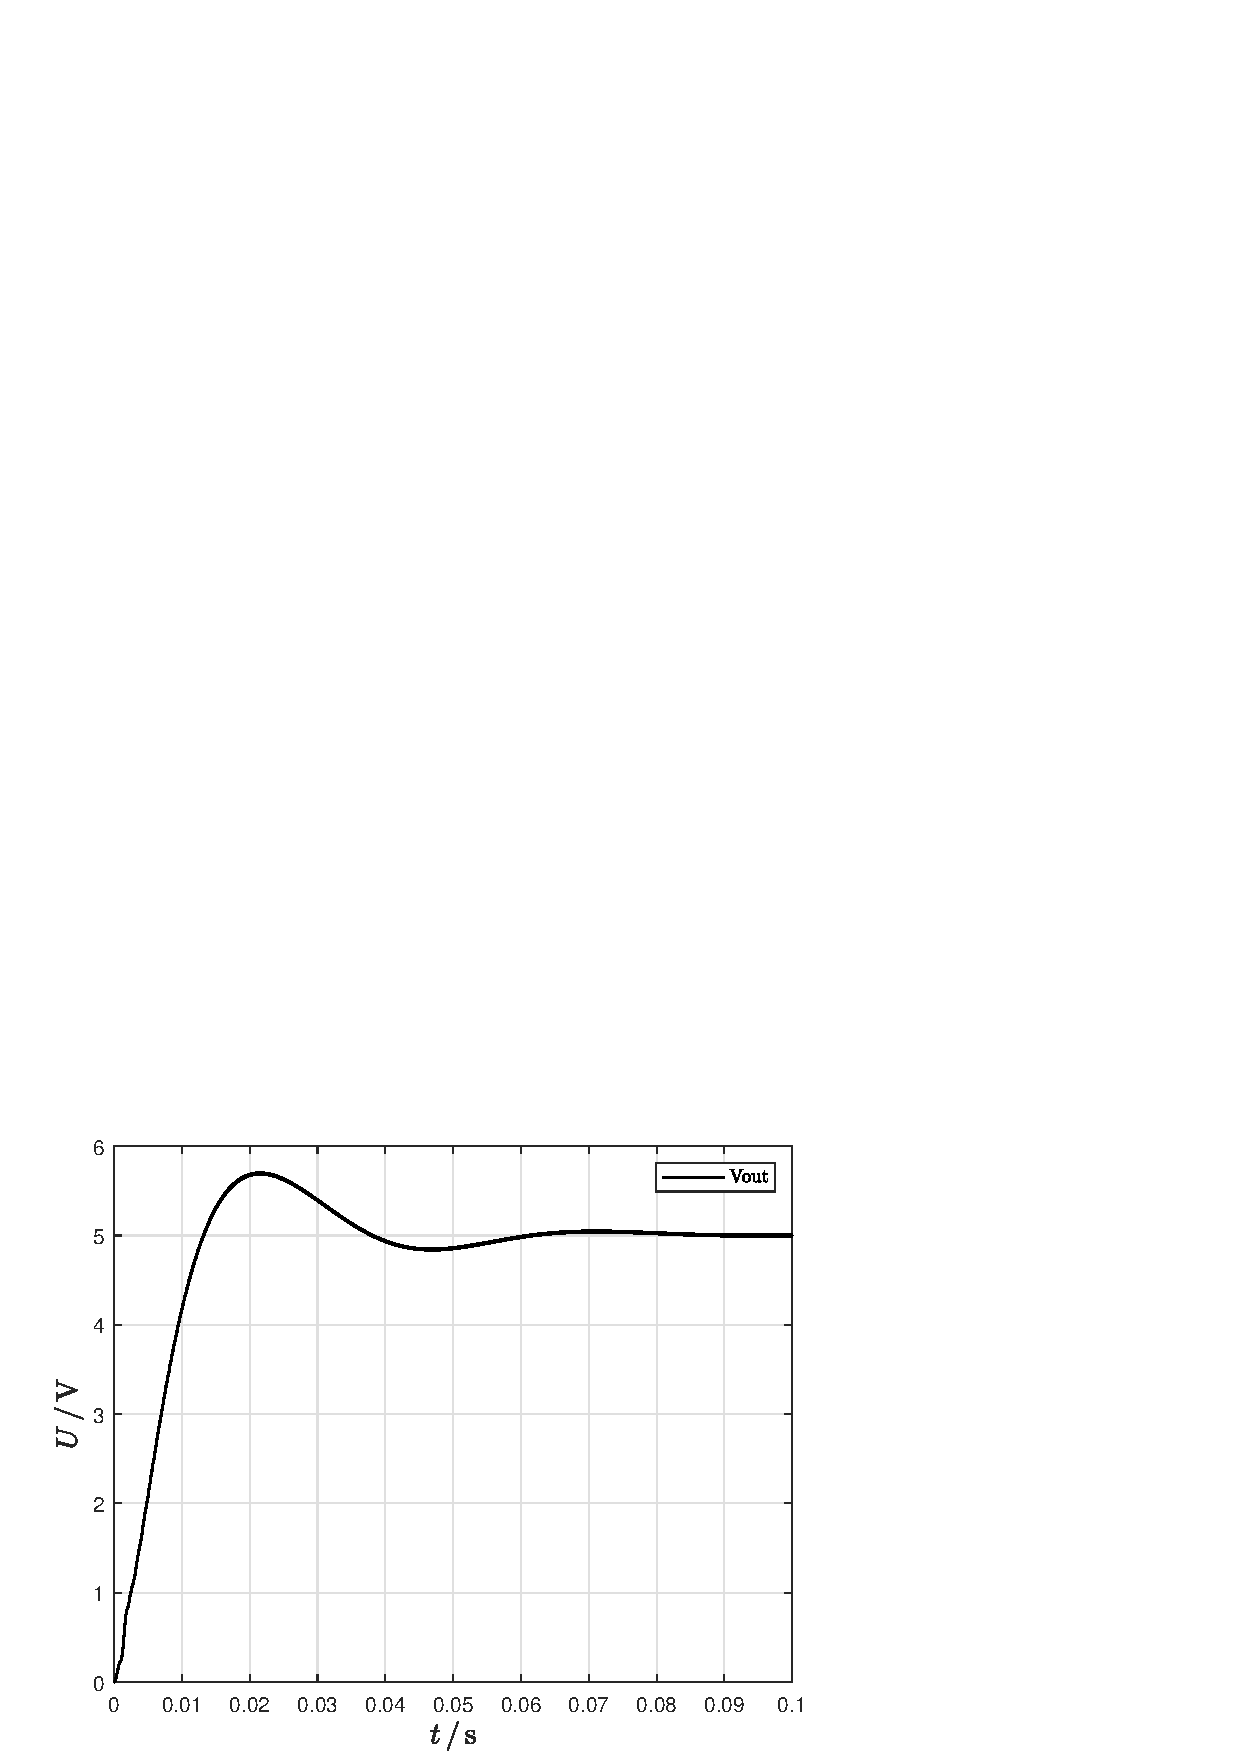
\includegraphics[width=0.8\linewidth]{Figure/Soft.png}
    \caption{FFT LTC3639 mit Filter}
    \label{fig:Soft}
\end{figure}

\begin{figure}[H]
    \centering
    \includegraphics[width=0.8\linewidth]{Figure/ControllerSoft.png}
    \caption{FFT LTC3639 mit Filter}
    \label{fig:ControllerSoft}
\end{figure}

\begin{figure}[H]
    \centering
    \includegraphics[width=0.8\linewidth]{Figure/SystemSoft.png}
    \caption{FFT LTC3639 mit Filter}
    \label{fig:SystemSoft}
\end{figure}

\subsection{PID Auslegung}

Ein besonderer Schwerpunkt lag auf der Auslegung eines PID-Reglers. Verschiedene Methoden zur Reglerparametrierung wurden getestet, darunter System Identification, State-Space-Modelle, Pole Placement und PID-Tuning. Keine dieser Methoden lieferte die gewünschten Ergebnisse. Auch die Übernahme von Parametern aus der Fachliteratur – z. B. aus dem Paper "Optimally Designed PID Controller for a DC-DC Buck Converter via a Hybrid Whale Optimization Algorithm with Simulated Annealing" – führte nicht zum Erfolg. Daher wurden die PID-Parameter empirisch angepasst, um eine stabile und performante Regelung zu gewährleisten. Die finalen Werte lauten:

\begin{itemize}
    \item Reglertyp: Discrete PI-Regler
    \item P-Anteil: 0.002
    \item I-Anteil: 7
\end{itemize}

\begin{figure}[H]
    \centering
    \includegraphics[width=0.8\linewidth]{Figure/DiscretPIDController_Parameter.png}
    \caption{FFT LTC3639 mit Filter}
    \label{fig:SystemSoft}
\end{figure}